\documentclass[egilmezThesis.tex]{subfiles} 
\begin{document}
\chapter{The New Approach}
\label{chap:MA}

As it was discussed and depicted, in chapter \ref{chap:Justification} the main problems of the previous approach are:
\begin{itemize}
\item Faulty inclusion of the credibility values for the fuzzy rules, into the similarity evaluation function.
\item The final result of the method converging to the default values defined between an arbitrary predicate and the identity predicate.
\item Flawed filtering mechanism of the search algorithm.
\item No means for utilizing the information which comes from shared similarity concepts in similarity predicate pairings.
\end{itemize}

Thus hereby we propose a new methodology which in general lines:
\begin{itemize}
\item Has a sound evaluation algorithm that prevents credibility values from dominating the final result.
\item Does not introduce any extra knowledge which is not originally in the knowledge base, so avoids problems like the final result converging to erroneous values.
\item Has a solid search algorithm which is able to utilize all of the information that the knowledge base contain, including similarity concepts that appear in more than one fuzzy rule.
\item And as the predicate trees are maintained in their original forms, algorithm is able to work effectively on the  complete structure emitting the need of filtering some parts of the data, which could potentially consist of crucial information.
\end{itemize}

We present the method in the following way:

We lay the fundamentals for a generic mathematical formulation of the main focus of the research. Then the application of the methodology in logic programming is inspected. Lastly, final section sheds light on the comparison of the current and prior approaches via observing solid examples.
%\begin{comment}

%\end{comment}

%\documentclass[Thesis.tex]{subfiles} 
\begin{document}

\chapter{Similarity of fuzzy logic}
\label{chap:Similarity}
\subsection{overview of similarity}
\label{sec:overview}
%\section{overview of similarity}
%\label{sec:overview} Not in Thesis
Similarity appears and is applied almost everywhere in our daily life. Natural language gives a lot of vivid examples. The adjective vocabularies to describe a pretty girl, could be `good-looking', `beautiful', `nice', `attractive', and even more can be found in Shakespeare's work or Oxford dictionary. The phenomenon that there is the semantic similarity among vocabularies is called synonym in linguistics research area. The well-known linguistic project containing the similarity idea is WordNet \cite{Fel98}, in which, nouns, verbs, adjectives and adverbs are grouped into sets of cognitive synonyms, each expressing a distinct concept. 

Not only just for mechanical fun in linguistic research, similarity is also widely used for the cognitive processes in the human mind, visual and acoustic perception, motor movements and imprecise and uncertain knowledge representation and approximate reasoning and games.

Since natural language is ambiguous and vague, the keyword you search for in searching engines on web are mostly imprecise. For example, if `old furniture' is the keyword typed, `old' should be considered as a fuzzy concept, since we don't know how `old' should be. It may retrieve the `classical furniture', `antique furniture', or may obtain the `second hand furniture', which is quite different from `classical furniture' and `antique furniture'. However, `classical', `antique', and `second hand' have certain different similarity with the word `old'. The search engines returns `classical furniture', `antique furniture' and `second hand furniture', and other results which are similar to the keywords `old'. Therefore, by the semantic similarity, the concept-related result is returned, which makes the search process imprecise, but in fact returns the expected results, since in reality, the interesting information a human being requires is not always accurate, but approximate, which makes similarity important and necessary in both research area and industrial engineering. 

Fuzzy Logic is used to represent vague information in the real world. In order to draw the similarity between objects in real world, we introduce similarity between predicates into Fuzzy Logic. Similarity itself is a fuzzy concept, which makes fuzzy logic suitable and appropriate for representing similarity. 

In order to embed similarity into \textit{Fuzzy Logic}, we focus on the similarity between predicates. The reasons are,

\begin{enumerate}
\item In Fuzzy Logic, term is presented to be an object in the interested domain. While predicate represents the fuzzy concept and mostly is interpreted as property of terms. The similarity between two objects is achieved by comparing their properties. Thus, comparing predicates is actually comparing the properties of objects.

\item In Fuzzy Logic, the atomic query is an atom, which is a predicate with its arguments. Obtaining the similarity between predicates,  is one approach to fruit similar queries, which leads to similar answers.
\end{enumerate}

\subsection{Structure of the paper}
%In this Chapter,
In this paper,  we present two approaches to obtain similarity between predicates. One is \textit{Interpretation\_Based Measurement} in section \ref{sec:IBM}, and another is presented in section \ref{sec:SBM}, called \textit{Structured\_Based Measurement}. We compare these two measurements in section \ref{sec:CompTwoMeasurements}. The conclusion is drawn in the final section.

\documentclass[Thesis.tex]{subfiles} 
\begin{document}

\chapter{Similarity of fuzzy logic}
\label{chap:Similarity}
\subsection{overview of similarity}
\label{sec:overview}
%\section{overview of similarity}
%\label{sec:overview} Not in Thesis
Similarity appears and is applied almost everywhere in our daily life. Natural language gives a lot of vivid examples. The adjective vocabularies to describe a pretty girl, could be `good-looking', `beautiful', `nice', `attractive', and even more can be found in Shakespeare's work or Oxford dictionary. The phenomenon that there is the semantic similarity among vocabularies is called synonym in linguistics research area. The well-known linguistic project containing the similarity idea is WordNet \cite{Fel98}, in which, nouns, verbs, adjectives and adverbs are grouped into sets of cognitive synonyms, each expressing a distinct concept. 

Not only just for mechanical fun in linguistic research, similarity is also widely used for the cognitive processes in the human mind, visual and acoustic perception, motor movements and imprecise and uncertain knowledge representation and approximate reasoning and games.

Since natural language is ambiguous and vague, the keyword you search for in searching engines on web are mostly imprecise. For example, if `old furniture' is the keyword typed, `old' should be considered as a fuzzy concept, since we don't know how `old' should be. It may retrieve the `classical furniture', `antique furniture', or may obtain the `second hand furniture', which is quite different from `classical furniture' and `antique furniture'. However, `classical', `antique', and `second hand' have certain different similarity with the word `old'. The search engines returns `classical furniture', `antique furniture' and `second hand furniture', and other results which are similar to the keywords `old'. Therefore, by the semantic similarity, the concept-related result is returned, which makes the search process imprecise, but in fact returns the expected results, since in reality, the interesting information a human being requires is not always accurate, but approximate, which makes similarity important and necessary in both research area and industrial engineering. 

Fuzzy Logic is used to represent vague information in the real world. In order to draw the similarity between objects in real world, we introduce similarity between predicates into Fuzzy Logic. Similarity itself is a fuzzy concept, which makes fuzzy logic suitable and appropriate for representing similarity. 

In order to embed similarity into \textit{Fuzzy Logic}, we focus on the similarity between predicates. The reasons are,

\begin{enumerate}
\item In Fuzzy Logic, term is presented to be an object in the interested domain. While predicate represents the fuzzy concept and mostly is interpreted as property of terms. The similarity between two objects is achieved by comparing their properties. Thus, comparing predicates is actually comparing the properties of objects.

\item In Fuzzy Logic, the atomic query is an atom, which is a predicate with its arguments. Obtaining the similarity between predicates,  is one approach to fruit similar queries, which leads to similar answers.
\end{enumerate}

\subsection{Structure of the paper}
%In this Chapter,
In this paper,  we present two approaches to obtain similarity between predicates. One is \textit{Interpretation\_Based Measurement} in section \ref{sec:IBM}, and another is presented in section \ref{sec:SBM}, called \textit{Structured\_Based Measurement}. We compare these two measurements in section \ref{sec:CompTwoMeasurements}. The conclusion is drawn in the final section.

\documentclass[Thesis.tex]{subfiles} 
\begin{document}

\chapter{Similarity of fuzzy logic}
\label{chap:Similarity}
\input{Content/Similarity/Content/Introduction/introduction}

\input{Content/Similarity/Content/Interpretation_Base/similarity}

\input{Content/Similarity/Content/Structure_Base/similarity}

\input{Content/Similarity/Content/Comparison/comparison}
\end{document}

\documentclass[Thesis.tex]{subfiles} 
\begin{document}

\chapter{Similarity of fuzzy logic}
\label{chap:Similarity}
\input{Content/Similarity/Content/Introduction/introduction}

\input{Content/Similarity/Content/Interpretation_Base/similarity}

\input{Content/Similarity/Content/Structure_Base/similarity}

\input{Content/Similarity/Content/Comparison/comparison}
\end{document}

\section{Comparison of two measurements}
\label{sec:CompTwoMeasurements}
In this section, we compare two measurements which are Interpretation Based Measurement (IBM) in section \ref{sec:IBM}, and  Structure Based Measurement (SBM) in section \ref{sec:SBM}. The comparison is drawn from three points, the intuitions, the methods, and the results of IBM and SBM.

\begin{itemize}
\item Intuition 

The similarity between predicates in Fuzzy Logic is to represent the similarity between objects in the real world. Therefore, the intuition begins with  the similarity between objects. In Interpretation Based Measurement (IBM), objects are considered to be represented as a set of attributes it possesses, and similarity between two objects is the commonality of attributes of them. In Structure Based Measurement (SBM), the definition of objects is the key to obtain similarity. It works like mathematical proof, starting with the basic definition. And in SBM, the definition of objects  is represented with structured property.

\item Methotology

By Intuition of IBM, the problem is formalized as the similarity between sets. We start with discussing the similarity between crisp sets, and generalizing into similarity between fuzzy sets. According to the corresponding relation between fuzzy set and Fuzzy Logic presented in Chapter \ref{chap:CorrespondingRelation}, the similarity between fuzzy predicates is deduced from similarity between fuzzy sets. The idea of SBM is from an interesting topic in \textit{Foundations of Databases} \cite{AHV95}, which is achieving subsumption and equivalence between queries. The method is to find the isomorphism between atoms in the bodies of two comparing queries. In SBM, fuzzy rule with fuzzy predicate as head are considered as the ``defintion" of this predicate. To obtain similarity between two predicates, we start with their ``definitions" which are fuzzy rules by finding the similarity between the predicates in their bodies. Since the ``definition" of predicate is defined inductively. The basic one is the predicate which never appears in the head of any fuzzy rules. The predicate is formalized as predicate tree. The similarity between predicates is obtaining by comparing predicate trees. The Algorithm is defined inductively with promising complexity, since inductive is a property of tree.

\item Result

From IBM, both \textit{essential similarity} and \textit{surficial similarity} are obtained. From intuition of IBM, we actually assume the statement `` if two objects have more attributes in common, then they are more similar to each other" is true. But the true statement should be ``if two objects are more similar, then they have more attributes in common." 
\textit{Essential similarity} and \textit{surficial similarity} satisfy the first statement, because that is the intuition of IBM, used to obtain the result. However, \textit{essential similarity} satisfies the second statement, but \textit{surficial similarity} doesn't. That is why we name it ``surficial". The result from SBM avoids the disadvantage in IBM, but if some basic similarity is not defined, the ``essential similarity" will not be shown in the result. For example, comparing $p_1$ and $p_2$, there are two atomic predicates $q_1$ and $q_2$ in their ``definition" respectively, they may be similar to each other, but if this similarity between $q_1$ and $q_2$ is not defined, the similarity between $p_1$ and $p_2$ will be affected, like ``distortion". Also, only predicates with the same type and their fuzzy rules with same connective can be compared, which limits the result of the essential similarity between fuzzy concepts.

\end{itemize}



\end{document}

\documentclass[Thesis.tex]{subfiles} 
\begin{document}

\chapter{Similarity of fuzzy logic}
\label{chap:Similarity}
\subsection{overview of similarity}
\label{sec:overview}
%\section{overview of similarity}
%\label{sec:overview} Not in Thesis
Similarity appears and is applied almost everywhere in our daily life. Natural language gives a lot of vivid examples. The adjective vocabularies to describe a pretty girl, could be `good-looking', `beautiful', `nice', `attractive', and even more can be found in Shakespeare's work or Oxford dictionary. The phenomenon that there is the semantic similarity among vocabularies is called synonym in linguistics research area. The well-known linguistic project containing the similarity idea is WordNet \cite{Fel98}, in which, nouns, verbs, adjectives and adverbs are grouped into sets of cognitive synonyms, each expressing a distinct concept. 

Not only just for mechanical fun in linguistic research, similarity is also widely used for the cognitive processes in the human mind, visual and acoustic perception, motor movements and imprecise and uncertain knowledge representation and approximate reasoning and games.

Since natural language is ambiguous and vague, the keyword you search for in searching engines on web are mostly imprecise. For example, if `old furniture' is the keyword typed, `old' should be considered as a fuzzy concept, since we don't know how `old' should be. It may retrieve the `classical furniture', `antique furniture', or may obtain the `second hand furniture', which is quite different from `classical furniture' and `antique furniture'. However, `classical', `antique', and `second hand' have certain different similarity with the word `old'. The search engines returns `classical furniture', `antique furniture' and `second hand furniture', and other results which are similar to the keywords `old'. Therefore, by the semantic similarity, the concept-related result is returned, which makes the search process imprecise, but in fact returns the expected results, since in reality, the interesting information a human being requires is not always accurate, but approximate, which makes similarity important and necessary in both research area and industrial engineering. 

Fuzzy Logic is used to represent vague information in the real world. In order to draw the similarity between objects in real world, we introduce similarity between predicates into Fuzzy Logic. Similarity itself is a fuzzy concept, which makes fuzzy logic suitable and appropriate for representing similarity. 

In order to embed similarity into \textit{Fuzzy Logic}, we focus on the similarity between predicates. The reasons are,

\begin{enumerate}
\item In Fuzzy Logic, term is presented to be an object in the interested domain. While predicate represents the fuzzy concept and mostly is interpreted as property of terms. The similarity between two objects is achieved by comparing their properties. Thus, comparing predicates is actually comparing the properties of objects.

\item In Fuzzy Logic, the atomic query is an atom, which is a predicate with its arguments. Obtaining the similarity between predicates,  is one approach to fruit similar queries, which leads to similar answers.
\end{enumerate}

\subsection{Structure of the paper}
%In this Chapter,
In this paper,  we present two approaches to obtain similarity between predicates. One is \textit{Interpretation\_Based Measurement} in section \ref{sec:IBM}, and another is presented in section \ref{sec:SBM}, called \textit{Structured\_Based Measurement}. We compare these two measurements in section \ref{sec:CompTwoMeasurements}. The conclusion is drawn in the final section.

\documentclass[Thesis.tex]{subfiles} 
\begin{document}

\chapter{Similarity of fuzzy logic}
\label{chap:Similarity}
\input{Content/Similarity/Content/Introduction/introduction}

\input{Content/Similarity/Content/Interpretation_Base/similarity}

\input{Content/Similarity/Content/Structure_Base/similarity}

\input{Content/Similarity/Content/Comparison/comparison}
\end{document}

\documentclass[Thesis.tex]{subfiles} 
\begin{document}

\chapter{Similarity of fuzzy logic}
\label{chap:Similarity}
\input{Content/Similarity/Content/Introduction/introduction}

\input{Content/Similarity/Content/Interpretation_Base/similarity}

\input{Content/Similarity/Content/Structure_Base/similarity}

\input{Content/Similarity/Content/Comparison/comparison}
\end{document}

\section{Comparison of two measurements}
\label{sec:CompTwoMeasurements}
In this section, we compare two measurements which are Interpretation Based Measurement (IBM) in section \ref{sec:IBM}, and  Structure Based Measurement (SBM) in section \ref{sec:SBM}. The comparison is drawn from three points, the intuitions, the methods, and the results of IBM and SBM.

\begin{itemize}
\item Intuition 

The similarity between predicates in Fuzzy Logic is to represent the similarity between objects in the real world. Therefore, the intuition begins with  the similarity between objects. In Interpretation Based Measurement (IBM), objects are considered to be represented as a set of attributes it possesses, and similarity between two objects is the commonality of attributes of them. In Structure Based Measurement (SBM), the definition of objects is the key to obtain similarity. It works like mathematical proof, starting with the basic definition. And in SBM, the definition of objects  is represented with structured property.

\item Methotology

By Intuition of IBM, the problem is formalized as the similarity between sets. We start with discussing the similarity between crisp sets, and generalizing into similarity between fuzzy sets. According to the corresponding relation between fuzzy set and Fuzzy Logic presented in Chapter \ref{chap:CorrespondingRelation}, the similarity between fuzzy predicates is deduced from similarity between fuzzy sets. The idea of SBM is from an interesting topic in \textit{Foundations of Databases} \cite{AHV95}, which is achieving subsumption and equivalence between queries. The method is to find the isomorphism between atoms in the bodies of two comparing queries. In SBM, fuzzy rule with fuzzy predicate as head are considered as the ``defintion" of this predicate. To obtain similarity between two predicates, we start with their ``definitions" which are fuzzy rules by finding the similarity between the predicates in their bodies. Since the ``definition" of predicate is defined inductively. The basic one is the predicate which never appears in the head of any fuzzy rules. The predicate is formalized as predicate tree. The similarity between predicates is obtaining by comparing predicate trees. The Algorithm is defined inductively with promising complexity, since inductive is a property of tree.

\item Result

From IBM, both \textit{essential similarity} and \textit{surficial similarity} are obtained. From intuition of IBM, we actually assume the statement `` if two objects have more attributes in common, then they are more similar to each other" is true. But the true statement should be ``if two objects are more similar, then they have more attributes in common." 
\textit{Essential similarity} and \textit{surficial similarity} satisfy the first statement, because that is the intuition of IBM, used to obtain the result. However, \textit{essential similarity} satisfies the second statement, but \textit{surficial similarity} doesn't. That is why we name it ``surficial". The result from SBM avoids the disadvantage in IBM, but if some basic similarity is not defined, the ``essential similarity" will not be shown in the result. For example, comparing $p_1$ and $p_2$, there are two atomic predicates $q_1$ and $q_2$ in their ``definition" respectively, they may be similar to each other, but if this similarity between $q_1$ and $q_2$ is not defined, the similarity between $p_1$ and $p_2$ will be affected, like ``distortion". Also, only predicates with the same type and their fuzzy rules with same connective can be compared, which limits the result of the essential similarity between fuzzy concepts.

\end{itemize}



\end{document}

\section{Comparison of two measurements}
\label{sec:CompTwoMeasurements}
In this section, we compare two measurements which are Interpretation Based Measurement (IBM) in section \ref{sec:IBM}, and  Structure Based Measurement (SBM) in section \ref{sec:SBM}. The comparison is drawn from three points, the intuitions, the methods, and the results of IBM and SBM.

\begin{itemize}
\item Intuition 

The similarity between predicates in Fuzzy Logic is to represent the similarity between objects in the real world. Therefore, the intuition begins with  the similarity between objects. In Interpretation Based Measurement (IBM), objects are considered to be represented as a set of attributes it possesses, and similarity between two objects is the commonality of attributes of them. In Structure Based Measurement (SBM), the definition of objects is the key to obtain similarity. It works like mathematical proof, starting with the basic definition. And in SBM, the definition of objects  is represented with structured property.

\item Methotology

By Intuition of IBM, the problem is formalized as the similarity between sets. We start with discussing the similarity between crisp sets, and generalizing into similarity between fuzzy sets. According to the corresponding relation between fuzzy set and Fuzzy Logic presented in Chapter \ref{chap:CorrespondingRelation}, the similarity between fuzzy predicates is deduced from similarity between fuzzy sets. The idea of SBM is from an interesting topic in \textit{Foundations of Databases} \cite{AHV95}, which is achieving subsumption and equivalence between queries. The method is to find the isomorphism between atoms in the bodies of two comparing queries. In SBM, fuzzy rule with fuzzy predicate as head are considered as the ``defintion" of this predicate. To obtain similarity between two predicates, we start with their ``definitions" which are fuzzy rules by finding the similarity between the predicates in their bodies. Since the ``definition" of predicate is defined inductively. The basic one is the predicate which never appears in the head of any fuzzy rules. The predicate is formalized as predicate tree. The similarity between predicates is obtaining by comparing predicate trees. The Algorithm is defined inductively with promising complexity, since inductive is a property of tree.

\item Result

From IBM, both \textit{essential similarity} and \textit{surficial similarity} are obtained. From intuition of IBM, we actually assume the statement `` if two objects have more attributes in common, then they are more similar to each other" is true. But the true statement should be ``if two objects are more similar, then they have more attributes in common." 
\textit{Essential similarity} and \textit{surficial similarity} satisfy the first statement, because that is the intuition of IBM, used to obtain the result. However, \textit{essential similarity} satisfies the second statement, but \textit{surficial similarity} doesn't. That is why we name it ``surficial". The result from SBM avoids the disadvantage in IBM, but if some basic similarity is not defined, the ``essential similarity" will not be shown in the result. For example, comparing $p_1$ and $p_2$, there are two atomic predicates $q_1$ and $q_2$ in their ``definition" respectively, they may be similar to each other, but if this similarity between $q_1$ and $q_2$ is not defined, the similarity between $p_1$ and $p_2$ will be affected, like ``distortion". Also, only predicates with the same type and their fuzzy rules with same connective can be compared, which limits the result of the essential similarity between fuzzy concepts.

\end{itemize}



\end{document}

\section{Problem Description}
\label{PD}

The first step for our approach is generalizing the research's main focus, finding the similarity proximity of two predicates via giving a mathematical foundation. As seen in chapter \ref{chap:Justification}, the solution of the problem relies heavily on the predefined similarity relations between subconcepts. Moreover it was displayed that by expanding the rules in the knowledge bases, the construction of the predicate trees resulted in a graph representation of the original domain. This problem of matching subconcepts in two trees can easily describe the precise meaning of the matching with a mathematical definition. Informally, one may define matching between two predicates in a knowledge base of a logic program as follows: given some specific node corresponding to concept of our interest in the knowledge base- call it \textit{a}, two concepts (i.e. \textit{a} and candidate node) can be matched in the corresponding trees if there is a mapping between some specific subset of nodes which are reachable from \textit{a} in first tree and some subset of nodes which are reachable from candidate node in the second tree. 

%\newpage
\subsection{Preliminaries}
\label{prem}
A function $f$ is a relation between a set of inputs and a set of permissible outputs with the property that each input is related to exactly one output.

A \textit{directed graph}  (digraph) is an ordered pair \textit{ (V, E)} , where V is a set and E is a binary relation on V .

In a digraph \textit{(V, E )}, the elements of \textit{V} are called vertices, and the elements of \textit{E} are called the edges of the digraph.

A digraph \textit{(V',E')} is a subgraph of a digraph \textit{(V, E )} if ${V'} \subseteq {V}$ and ${E'} 
\subseteq {E}.$

In a digraph $(V,E)$, a path from a vertex $u$ to a vertex $u'$ is a sequence $\langle v_0,v_1,... ,v_k \rangle$ of vertices such that $u=v_0$ and $u' =v_k$,and $(v_{i-1},v_i)  \in E$ for $1 \leq i \leq k$; we call $v_k$ as the terminal node of the path. If there is a path from a vertex $u$ to a vertex $v$, then we say that $v$ is reachable from $u$. If $V�$ is a subset of $V$, a path from $u$ to $v$ whose vertices belong to $V'$ is a path from $u$ to $v$ in $V'$. If there exists a path from $u$ to $v$ in $V'$ , $v$ is reachable from $u$ in $V'$.

Let $G_0 = (V_0,E_0)$ be a digraph whose vertices are labeled by a function $f_0 : V_0 \to VL_0$ where $VL_0$ is the vertex labels of $G_0$ and let $G_1 = (V_1,E_1)$ be a graph whose vertices are labeled by a function $f_1 : V_1 \to VL_1$ where $VL_1$ is the vertex labels of $G_1$. Let $vm$ be a function that maps the label of a vertex in $VL_0$ to a set of vertex labels in $VL_1$.

We say that a  terminal node $v_0$ matches a terminal node $v_1$, iff \\ \begin{center} $VL_1(v_1) \in vm(VL_0(v_0))$. \end{center}
Informally a  terminal node $v_0$ matches a terminal node $v_1$, when the vertex label of $v_1$ is in the vertex label set that the vertex label of $v_0$ is mapped to by $vm$.

We say that an arbitrary node $v_0$ matches an arbitrary node $v_1$, iff \begin{center}
\textit{For each element  $u_0$ of a subset of vertices reachable from $v_0$ via a path $p_0$, there exists a vertex $u_1$ reachable from $v_1$ via a path $p_1$ in $G_1$ such that $u_0$ matches $u_1$.} \end{center}

Again if we are to state the meaning in an informal manner, two arbitrary nodes $v_0$ and $v_1$ match, if and only if there exists a set of vertices that are reachable from $v_0$, and each of these vertices match to some vertex which are reachable from $v_1$.

\subsection{Vertex Matching Problem}
\label{MP}
We define an Vertex Matching Problem \emph{(VMP)} with the following input:
\begin{itemize}
	\item Two finite, polynomially bounded directed graphs: $G_0=(V_0, E_0)$, $G_1=(V_1, E_1)$
	\item Vertex Labeling Functions: $f_0: V_0 \rightarrow VL_0$, $f_1: V_1 \rightarrow VL_1$
  \item  Vertex Labeling Match Function: $vm: VL_0 \rightarrow 2^{VL_1}$
  \item Vertices to be matched: $v_0 \in V_0$, $v_1 \in V_1$
 \end{itemize}

\section{Algorithm in the Domain of Fuzzy Logic}
\label{algFL}

The application of the generic formalism presented in section \ref{PD} consists of three steps:
\begin{itemize}
\item Construction of the predicate tree
\item Search algorithm for similar predicates
\item The similarity evaluation function
\end{itemize}

In a nutshell, firstly the predicate trees are constructed via utilizing the fuzzy rules of the program. Then the search algorithm locates similar predicate pairings and collects the corresponding values. Finally the evaluation algorithm computes the resulting similarity proximity value for the predicate pair of interest.

The topics are inspected in detail in the following subsections respectively.

\subsection{Construction of the Predicate Tree}
\label{eval}

The process for building the predicate trees follow the same methodology as the one depicted in section \ref{sec:Construct}. Thus as a brief recap we might state that, for every fuzzy rule in the knowledge base in the following form:

\[p_{c}(\vec{t}) \stackrel{c,F_c}{\longleftarrow}F(p_1(\vec{t_1}),...,p_n(\vec{t_n}))\] 

we expand the head of the rule $p_c$ via adding the predicates that the body of the fuzzy rule contain, i.e. $p_1, ..., p_n$, as its children in the directed tree graph. The task continues in a recursive manner until all the rules are exhausted. 

No modifications are done on the original predicate trees at any step of the algorithm. Hence the process of building the trees is very straightforward.



\subsection{Search and Evaluation}
\label{SandE}

Similarity searching process heavily builds on the generic  \textit{vertex matching algorithm} given in section \ref{PD}. The only modification is that instead of searching exact matches between the subconcepts, the focus is on finding ones for which a fuzzy similarity rule exists in the particular program.

So if we are to re-state the methodology with the minor modification, when observing the similarity between predicates \textit{$p_{1}$} and \textit{$p_{2}$}, for every vertex \textit{$v_{1}$} reachable from \textit{$p_{1}$} via a path \textit{$t_{1}$}, the algorithm looks for a vertex \textit{$v_{2}$} reachable from \textit{$p_{2}$} via a path \textit{$t_{2}$} where the similarity degree between \textit{$v_{1}$}  and \textit{$v_{2}$} is defined. The values of these relations are collected in the set \textit{sm} and similarity degree \textit{sd} between \textit{$p_{1}$} and \textit{$p_{2}$} is evaluated with the following equation:

\begin{equation}\label{eq:sd}
\textit{$sd(p_{1}, p_{2})$} =   (1-\lvert  \textit{$cred_{p_{1}}$} - \textit{$cred_{p_{2}}$}  \rvert) \textbf{\emph{OP}} (\frac{\sum_{i=1}^{n} sm_i}{n})
\end{equation}

where $cred_{1}$ and  $cred_{2}$ are the credibility values of the fuzzy rules that contain \textit{$p_{1}$} and \textit{$p_{2}$} in their heads respectively, \textit{$OP$} is the fuzzy operator that is again defined by those rules, and  \textit{$n$} is the cardinality of the set \textit{sm}.

Mind that as the focus is on two fuzzy rules at a given time, there might me two distinct \textit{$OP$} values for the corresponding rules. In those cases, the generic product operation defined on real number is taken as the default \textit{$OP$} value.

\section{Improvements Over Related Work}
\label{Improvements}

The purpose of the section is depicting the contributions the new methodology introduces, specifically the improvements over the related work, the \textit{Structured Based Measurement} that was introduced by Lu \cite{Lu}.  As mentioned in the beginning of this chapter, main sources of advancement are the way the predicate trees are constructed, the methodology for searching the predicate trees, and the structure of the evaluation algorithm. We will re-visit the examples that had been presented in chapter \ref{chap:Justification} in order to observe how the new methodology compare to \textit{SBM} and also see some extension that it introduces to the domain of interest which gives birth to some interesting features for the framework.



\subsection{Inclusion of Credibilities in Similarity Evaluation Function}
\label{cred2}

The first difference of the approaches come with the way they utilize the credibility values of the fuzzy rules in the similarity evaluation function for the predicates. As mentioned in the previous chapter, the way that \textit{SBM} adopts proves to be problematic when the branching factor is small.  Since it's directly summed with the values of similarity pairs in the numerator of the equation, when the cardinality \textit{n} is small, the values of credibilities simply overshadow of similarity pairs.

\begin{ex}
The following simple example displays one such scenario:

\begin{center}
\begin{tabular}{l l}
$good\_basketball\_player:$  & $(Player)$\\

$bad\_basketball\_player:$ &  $(Player)$\\

$good\_technique:$ &  $(Player)$\\

$egoism:$ &  $(Player)$\\

\end{tabular}
\end{center}
\begin{tabular}{l l l}
$good\_basketball\_player(X)$ & $\stackrel{0.95,.}{\longleftarrow} prod$ & $good\_technique(X)$.\\

$bad\_basketball\_player(X)$ & $\stackrel{0.9,.}{\longleftarrow} prod$ & $egoism(X)$ .\\

\end{tabular}
\[Sim(good\_technique, egoism) = 0.1\]

\end{ex}

The predicate trees are the same for both of the approaches since there is no need for expansion in this case as they're structurally equivalent. The built trees are as follows: 



\begin{figure}[h!]
\begin{center}
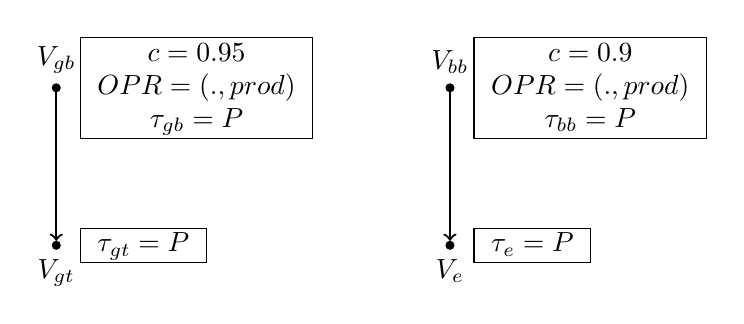
\begin{tikzpicture}[yscale=-1,
place/.style={circle,draw=black, fill=black, inner sep=0pt, 
              minimum size=1mm}]

\node[place] (1st) at (0, 0) [label=above: $V_{gb}$,
                              label=right: {
             \begin{tabular}{|c|}
               \hline
               $c=0.95$ \\
               $OPR=(.,prod)$ \\
               $\tau_{gb}=P$ \\
               \hline
             \end{tabular} }] {};

\node[place] (2nd) at (0, 2) [label=below:  $V_{gt}$,
                                label=right: {
             \begin{tabular}{|c|}
               \hline
               $\tau_{gt}=P$\\
               %\textit{atmic mark} $0$ \\
               \hline
             \end{tabular} }
] {};
        
	\draw[->, thick] (1st) -- (2nd);

\begin{scope}[xshift=5cm]
 \node[place] (1st) at (0, 0) [label=above: $V_{bb}$,
                              label=right: {
             \begin{tabular}{|c|}
               \hline
               $c=0.9$ \\
               $OPR=(.,prod)$ \\
               $\tau_{bb}=P$ \\
               \hline
             \end{tabular} }] {};

\node[place] (2nd) at (0, 2) [label=below:  $V_{e}$,
                                label=right: {
             \begin{tabular}{|c|}
               \hline
               $\tau_{e}=P$\\
              % \textit{atomic mark} $0$\\
               \hline
             \end{tabular} }
] {};
        
	\draw[->, thick] (1st) -- (2nd);
\end{scope}

\end{tikzpicture}
\end{center}
\caption{Predicate trees for \textit{good\_basketball\_player} and \textit{bad\_basketball\_player}}
\label{fig:ExpansionTrHtf2}   
\end{figure}




By inspecting the example, one should \textbf{not} expect the predicates \textit{good\_basketball\_player} and \textit{bad\_basketball\_player} to be similar at all.

This is indeed the case for our approach.  Let us evaluate the similarity equation in order to demonstrate this:

In addition to the variables of the equation, we display the similar predicate pairs collected via the search algorithm in the set $pm$.

$cred_{p_{1}}$ = 0.95 , $cred_{p_{2}}$ = 0.9,  \emph{OP} = \textit{prod},  \textit{pm} = \{ (good\_technique, egoism)\},  \textit{sm} = \{\textit{0.1}\}, \textit{n} = 1.

When the values are input in the equation:


\begin{equation}\label{eq:sdE2}
\begin{split}
\textit{$sd(p_{1}, p_{2})$} &=   (1-\lvert  \textit{$cred_{p_{1}}$} - \textit{$cred_{p_{2}}$}  \rvert) \textbf{\emph{OP}} (\frac{\sum_{i=1}^{n} sm_i}{n})\\
&=   (1-\lvert  0.95 - 0.9  \rvert) . (\frac{0,1}{1}) \\
&= 0.095\\
&\cong{\textbf{0.1}}
 \end{split} 
\end{equation}

Our method evaluates  \textit{good\_basketball\_player} and \textit{bad\_basketball\_player}  as not similar, which is what we expect by using common sense. In contrast with that, as seen before, \textit{SBM} produces unexpected results. To illustrate this affirmation we show the results \textit{SBM} obtains:

$M_{s}$ = \{ (good\_technique, egoism)\}, $c^a$ = 0.95, $c^b$ = 0.9,   \textit{n} = 1.     

\begin{equation}\label{eq:sbmE2}
\begin{split}
M_v &=\frac{\sum_{i=1}^{1} v_i+1-\lvert c^a-c^b\rvert}{n+1}\\
&=\frac{0.1 +1-\lvert 0.95 - 0.9\rvert}{1+1}\\
&= \frac{1.05}{2}\\
&\cong{\textbf{0.53}}
 \end{split} 
\end{equation}

So on contrary to what was expected, \textit{SBM} calculated \textit{good\_basketball\_player} and \linebreak[4] \textit{bad\_basketball\_player} to be somewhat similar. As mentioned earlier, this problem is caused by the fact that the equation does not integrate the credibility values in a proper way, thus in some cases(when the branching factor is low) the emphasize is so high that it dominates the similarity values between the subpredicates. 

As displayed by the example, our approach handles this issue without any problems as it introduces the confidence values via the operator that is defined by the fuzzy rules themselves.


\subsection{Convergence to Identity Predicate}
\label{conv2}
We had stated that in order to compare two predicates, \textit{SBM} needs them to have the same tree structure. And in order to accomplish this when they are not equal, the missing branches and leaves of the smaller tree are filled with identity predicates. Moreover a default similarity value is defined between an arbitrary predicate and the identity predicate. 

In the same sense that it was discussed earlier, regrettably this introduces a couple of problems concerning the precision of the algorithm's final result. Similar to the effect that credibility values had in the previous section, this time we may have such an overwhelming impact from the default similarity values that is defined between the identity predicate and an arbitrary predicate.  We will especially encounter this kind of scenarios when one tree has high branching factor compared to the other one.


\begin{ex}
Once more we may see an example for that kind of case in the following program:
\begin{center}
\begin{tabular}{l l}
$classy\_restaurant:$  & $(Restaurant)$\\

$good\_restaurant:$  & $(Restaurant)$\\

$well\_trained\_waiters:$  & $(Restaurant)$\\

$expensive\_inventory:$  & $(Restaurant)$\\

$has\_good\_service:$  & $(Restaurant)$\\

$has\_healthy\_food:$  & $(Restaurant)$\\

$has\_tasty\_food:$  & $(Restaurant)$\\

$has\_nice\_surroundings:$  & $(Restaurant)$\\

$has\_high\_reputation:$  & $(Restaurant)$\\

\end{tabular}
\end{center}
\begin{tabular}{l l l}
$classy\_restaurant(X)$ & $\stackrel{1.0,.}{\longleftarrow} prod$ & $well\_trained\_waiters(X), expensive\_inventory(X).$\\

$good\_restaurant(X)$ & $\stackrel{0.95,.}{\longleftarrow} prod$ & $has\_healthy\_food(X), has\_good\_service(X),$\\ 
%$has\_nice\_surroundings(X), $ & $has\_nice\_surroundings(X),$ $has\_nice\_surroundings(X), $\\
$ $ & $$ & $has\_nice\_surroundings(X), has\_high\_reputation(X),$\\
$ $ & $$ & $has\_tasty\_food(X).$\\

\end{tabular}
\[Sim(well\_trained\_waiters, has\_good\_service) = 0.9\]
\[Sim(expensive\_inventory, has\_nice\_surroundings) = 0.8\]
\end{ex}

Regarding to the program we should expect the predicates \textit{classy\_restaurant} and \linebreak[4] \textit{good\_restaurant} to have a high similarity degree.

Again let's start evaluating the result with our new approach. Our algorithm does not require the predicates to be expanded so the tree are in their original form.

 \begin{figure}[h!]
\begin{center}
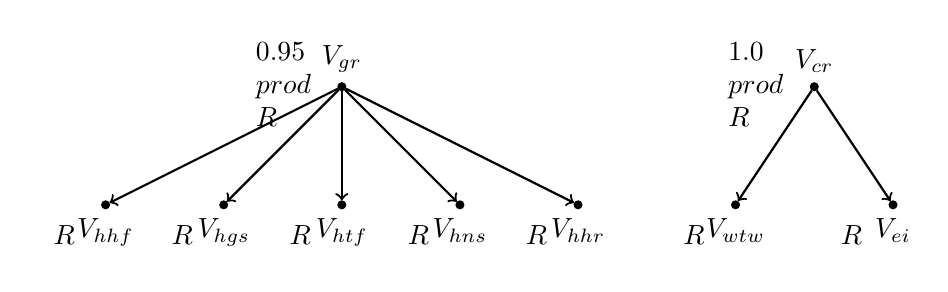
\begin{tikzpicture}[yscale=-1,
place/.style={circle,draw=black, fill=black, inner sep=0pt, 
              minimum size=1mm}]

  \node[place] (1st) at (3, 0) [label=above: $V_{gr}$,
                                  label=left: 
     \begin{tabular}{l}
        $0.95$\\
        $prod$\\
        $R$\\  
     \end{tabular}
] {};
  \node[place] (2nd) at (0, 1.5) [label=below: $V_{hhf}$,
                                  label=left:
     \begin{tabular}{l}
        $$\\
        $$\\
        $R$\\  
     \end{tabular}
]{};
  \node[place] (3rd) at (1.5, 1.5)  [label=below: $V_{hgs}$,
                                  label=left:
     \begin{tabular}{l}
        $$\\
        $$\\
        $R$\\  
     \end{tabular}	] {}; 
  \node[place] (4th) at (3, 1.5)   [label=below: $V_{htf}$,
                                  label=left:
     \begin{tabular}{l}
        $$\\
        $$\\
        $R$\\  
     \end{tabular}
             ] {}; 
             
 \node[place] (5th) at (4.5, 1.5) [label=below: $V_{hns}$,
                                  label=left:
     \begin{tabular}{l}
        $$\\
        $$\\
        $R$\\  
     \end{tabular}
             ] {}; 
             
             
   \node[place] (6th) at (6, 1.5)  [label=below: $V_{hhr}$,
                                  label=left:
     \begin{tabular}{l}
        $$\\
        $$\\
        $R$\\  
     \end{tabular}
             ] {};     

  %\node (dots) at (2,1.5) {$\cdots$};
	
  \draw[->, thick] (1st) -- (2nd);
  \draw[->, thick] (1st) -- (3rd);
  \draw[->, thick] (1st) -- (4th);
  \draw[->, thick] (1st) -- (5th);
  \draw[->, thick] (1st) -- (6th);

\begin{scope}[xshift=8cm]
  \node[place] (1st) at (1, 0) [label=above: $V_{cr}$,
                                  label=left: 
     \begin{tabular}{l}
        $1.0$\\
        $prod$\\
        $R$\\  
     \end{tabular}
] {};
  \node[place] (2nd) at (0, 1.5) [label=below: $V_{wtw}$,
                                  label=left:
     \begin{tabular}{l}
        $$\\
        $$\\
        $R$\\  
     \end{tabular}             ] {};
  \node[place] (3rd) at (2, 1.5) [label=below: $V_{ei}$,
                                  label=left:
     \begin{tabular}{l}
        $$\\
        $$\\
        $R$\\  
     \end{tabular}
             ] {}; 

%  \node (dots) at (1,1.5) {$\cdots$};
	
  \draw[->, thick] (1st) -- (2nd);
  \draw[->, thick] (1st) -- (3rd);
\end{scope}

);
\end{tikzpicture}
\end{center}
\caption{Predicate trees in original form}
\label{fig:res2}
\end{figure}


Then the values for the variables of the equation:

$cred_{p_{1}}$ = 0.95 , $cred_{p_{2}}$ = 1,  \emph{OP} = \textit{prod},  \textit{pm} = \{ (well\_trained\_waiters, has\_good\_service), (expensive\_inventory, has\_nice\_surroundings)\}, \textit{sm} = \{\textit{0.9, 0.8}\}, \textit{n} = 2.

And finally the evaluation:

\begin{equation}\label{eq:sdE3}
\begin{split}
\textit{$sd(p_{1}, p_{2})$} &=   (1-\lvert  \textit{$cred_{p_{1}}$} - \textit{$cred_{p_{2}}$}  \rvert) \textbf{\emph{OP}} (\frac{\sum_{i=1}^{n} sm_i}{n})\\
 &=   (1-\lvert  0.95 - 1  \rvert) . (\frac{0.9 + 0.8}{2}) \\
&\cong{\textbf{0.81}}
 \end{split} 
\end{equation}

As the result seems high enough in harmony with the expectation, indeed we can be satisfied with the evaluated degree of similarity. 

Thus we may pursue by constructing the predicate trees for  \textit{SBM}. As the two trees are not structurally equal, the smaller tree, the predicate tree of \textit{classy\_restaurant} must be expanded.



 \begin{figure}[h!]
\begin{center}
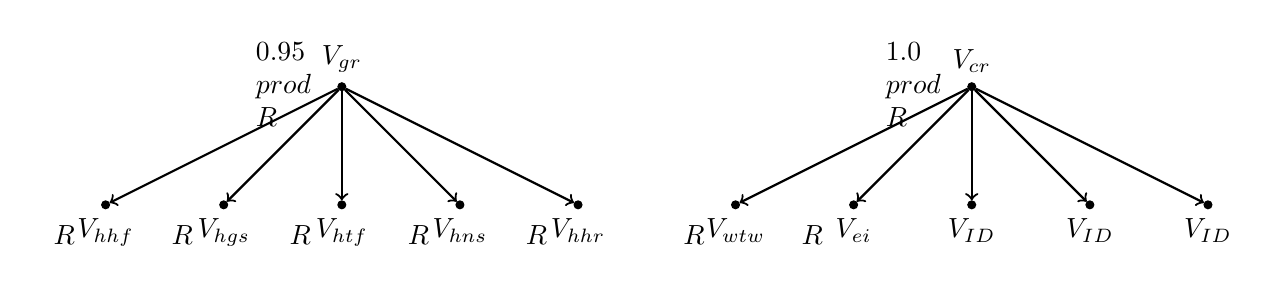
\begin{tikzpicture}[yscale=-1,
place/.style={circle,draw=black, fill=black, inner sep=0pt, 
              minimum size=1mm}]

  \node[place] (1st) at (3, 0) [label=above: $V_{gr}$,
                                  label=left: 
     \begin{tabular}{l}
        $0.95$\\
        $prod$\\
        $R$\\  
     \end{tabular}
] {};
  \node[place] (2nd) at (0, 1.5) [label=below: $V_{hhf}$,
                                  label=left:
     \begin{tabular}{l}
        $$\\
        $$\\
        $R$\\  
     \end{tabular}
]{};
  \node[place] (3rd) at (1.5, 1.5)  [label=below: $V_{hgs}$,
                                  label=left:
     \begin{tabular}{l}
        $$\\
        $$\\
        $R$\\  
     \end{tabular}	] {}; 
  \node[place] (4th) at (3, 1.5)   [label=below: $V_{htf}$,
                                  label=left:
     \begin{tabular}{l}
        $$\\
        $$\\
        $R$\\  
     \end{tabular}
             ] {}; 
             
 \node[place] (5th) at (4.5, 1.5) [label=below: $V_{hns}$,
                                  label=left:
     \begin{tabular}{l}
        $$\\
        $$\\
        $R$\\  
     \end{tabular}
             ] {}; 
             
             
   \node[place] (6th) at (6, 1.5)  [label=below: $V_{hhr}$,
                                  label=left:
     \begin{tabular}{l}
        $$\\
        $$\\
        $R$\\  
     \end{tabular}
             ] {};     

  %\node (dots) at (2,1.5) {$\cdots$};
	
  \draw[->, thick] (1st) -- (2nd);
  \draw[->, thick] (1st) -- (3rd);
  \draw[->, thick] (1st) -- (4th);
  \draw[->, thick] (1st) -- (5th);
  \draw[->, thick] (1st) -- (6th);

\begin{scope}[xshift=8cm]
  \node[place] (1st) at (3, 0) [label=above: $V_{cr}$,
                                  label=left: 
     \begin{tabular}{l}
        $1.0$\\
        $prod$\\
        $R$\\  
     \end{tabular}
] {};

  \node[place] (2nd) at (0, 1.5) [label=below: $V_{wtw}$,
                                  label=left:
     \begin{tabular}{l}
        $$\\
        $$\\
        $R$\\  
     \end{tabular}
]{};
  \node[place] (3rd) at (1.5, 1.5)  [label=below: $V_{ei}$,
                                  label=left:
     \begin{tabular}{l}
        $$\\
        $$\\
        $R$\\  
     \end{tabular}	] {}; 
  \node[place] (4th) at (3, 1.5)   [label=below: $V_{ID}$,
                                  label=left:
     \begin{tabular}{l}
        $$\\
        $$\\
       % $R$\\  
     \end{tabular}
             ] {}; 
             
 \node[place] (5th) at (4.5, 1.5) [label=below: $V_{ID}$,
                                  label=left:
     \begin{tabular}{l}
        $$\\
        $$\\
      %  $R$\\  
     \end{tabular}
             ] {}; 
             
             
   \node[place] (6th) at (6, 1.5)  [label=below: $V_{ID}$,
                                  label=left:
     \begin{tabular}{l}
        $$\\
        $$\\
   %     $R$\\  
     \end{tabular}
             ] {};     

%  \node (dots) at (1,1.5) {$\cdots$};
	
\draw[->, thick] (1st) -- (2nd);
  \draw[->, thick] (1st) -- (3rd);
  \draw[->, thick] (1st) -- (4th);
  \draw[->, thick] (1st) -- (5th);
  \draw[->, thick] (1st) -- (6th);
\end{scope}

);
\end{tikzpicture}
\end{center}
\caption{Predicate trees in expanded form for \textit{SBM}}
\label{fig:res2}
\end{figure}

There is just one level of expansion. Since at every level the $M_{s}$ that leads to the highest degree of similarity is chosen, the corresponding decision set will be: $M_{ds}$ = \textit{\{ (well\_trained\_waiters, has\_good\_service), (expensive\_inventory, has\_nice\_surroundings), (ID, has\_healthy\_food), (ID, has\_tasty\_food), (ID, has\_high\_reputation)\}}

One thing that we should pay attention to is that, since in this example, \textit{SBM} needed the introduction of the \textit{Identity Predicate}, a default similarity value  between an arbitrary predicate and the identity predicate should also be defined. Assume \textit{Sim(ID, p) = 0.3} for any arbitrary predicate.  

The rest of the variable values are as follows:

$c^a$ = 0.95, $c^b$ = 1,   \textit{n} = 5.     

\begin{equation}\label{eq:sbmE3}
\begin{split}
M_v &=\frac{\sum_{i=1}^{5} v_i+1-\lvert c^a-c^b\rvert}{n+1}\\
&=\frac{2.9 +1-\lvert 0.95 - 1\rvert}{5+1}\\
%&= \frac{1.05}{2}\\
&\cong{\textbf{0.55}}
 \end{split} 
\end{equation}

In this case the algorithm was not able to successfully evaluate and conclude that the predicates are actually closely related. This distortion was caused because of the relatively big branching factor difference and the identity predicates introduced for the missing one. As one can see, in \textit{SBM} as \textit{\textbf{the missing number of nodes in one tree increases,  the similarity degree calculated by the algorithm converges to the default values}} that is defined between an arbitrary predicate and the identity predicate.

Since our algorithm does not introduce any such external knowledge, and just use the original information of the knowledge base, it does not have such shortcomings.













\subsection{Wrong Filtering}
\label{filt2}

As one may remember from the earlier discussions from the previous chapter, there is one other faulty behavior of \textit{SBM} which we suspect to  be caused from the relaxed assumption of the knowledge bases. After every level of expansion, \textit{SBM} checks every predicate pair between the two trees with respect to their resulting similarity degree. Before the next level of expansion is pursued, a filtering is done on the tree by selecting the best pair combination on the level. The problem with this approach is that the information on a prior level is incomplete, and thus wrong steps can be taken when filtering that will cause the loss of crucial information for the main focus, \textit{i.e}. comparing the similarity values of the main predicates.  

Since the previous thesis work does not include any examples with predicate trees deeper then just one level, we try to demonstrate the problem with the following example:




\begin{ex}
The program consists of following type declarations and rules:

\begin{center}
\begin{tabular}{l l}

$modern\_city:$  & $(City)$\\

$livable\_city:$  & $(City)$\\

$life\_expectancy:$  & $(Society)$\\

$birth\_rate:$  & $(Society)$\\

$social\_welfare:$  & $(Society)$\\

$\#of\_schools$  & $(Society)$\\

$quality\_of\_academic\_staff$  & $(Society)$\\

$\#of\_teachers$  & $(Society)$\\

$compulsory\_schooling\_length$  & $(Society)$\\

$educated\_society:$  & $(Society)$\\

$\#of\_healthy\_individuals$  & $(Society)$\\

$literacy\_rate:$  & $(Society)$\\

$high\_population:$  & $(Society)$\\



\end{tabular}
\end{center}
\begin{tabular}{l l l}
$livable\_city(X)$ & $\stackrel{0.8,.}{\longleftarrow} prod$ & $literacy\_rate(X), \#of\_healthy\_individuals(X).$\\

$literacy\_rate(X)$ & $\stackrel{1.0,.}{\longleftarrow} prod$ & $compulsory\_schooling\_length(X), \#of\_teachers(X).$\\

$modern\_city(X)$ & $\stackrel{0.7,.}{\longleftarrow} prod$ & $educated\_society(X), high\_population(X),$\\ $$ & $$ & $social\_welfare(X).$\\ 
%$has\_nice\_surroundings(X), $ & $has\_nice\_surroundings(X),$ $has\_nice\_surroundings(X), $\\
%$ $ & $$ & $has\_nice\_surroundings(X), has\_high\_reputation(X).$\\
$educated\_society(X)$ & $\stackrel{1.0,.}{\longleftarrow} prod$ & $\#of\_schools(X), quality\_of\_academic\_staff(X).$\\ 
$high\_population(X)$ & $\stackrel{1,0,.}{\longleftarrow} prod$ & $birth\_rate(X), life\_expectancy(X).$\\ 


\end{tabular}
\[Sim(compulsory\_schooling\_length, \#of\_schools) = 0.9\]
\[Sim(\#of\_teachers, quality\_of\_academic\_staff) = 0.85\]
\[Sim(literacy\_rate, social\_welfare) = 0.4\]
\[Sim(\#of\_healthy\_individuals, life\_expectancy) = 0.7\]
\end{ex}


Focus of interest is evaluating the similarity degree of \textit{livable\_city} and \textit{modern\_city}. Let's start calculating this value via the new algorithm.



\begin{figure}[h!]
\begin{center}
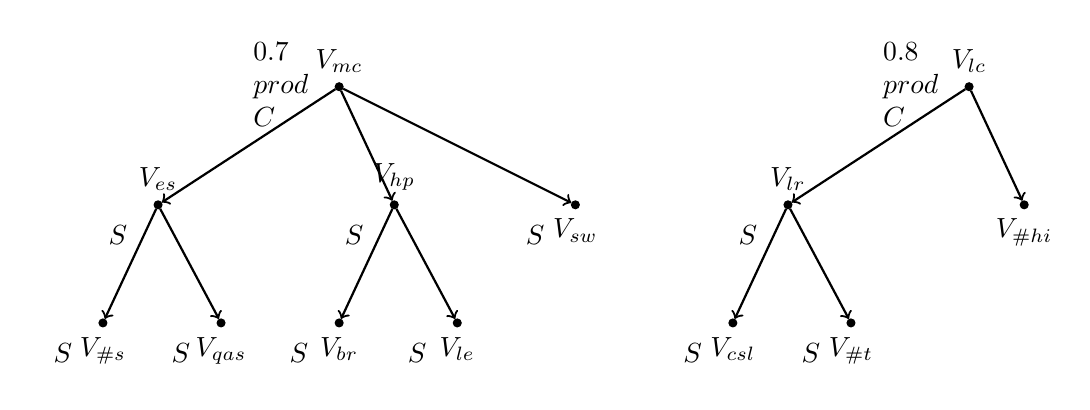
\begin{tikzpicture}[yscale=-1,
place/.style={circle,draw=black, fill=black, inner sep=0pt, 
              minimum size=1mm}]

  \node[place] (1st) at (3, 0) [label=above: $V_{mc}$,
                                  label=left: 
     \begin{tabular}{l}
        $0.7$\\
        $prod$\\
        $C$\\  
     \end{tabular}
] {};
  \node[place] (2nd) at (0.7, 1.5) [label=above: $V_{es}$,
                                  label=left:
     \begin{tabular}{l}
        $$\\
        $$\\
        $S$\\  
     \end{tabular}
]{};
  \node[place] (3rd) at (3.7, 1.5)  [label=above: $V_{hp}$,
                                  label=left:
     \begin{tabular}{l}
        $$\\
        $$\\
        $S$\\  
     \end{tabular}	] {}; 
  \node[place] (4th) at (6, 1.5)   [label=below: $V_{sw}$,
                                  label=left:
     \begin{tabular}{l}
        $$\\
        $$\\
        $S$\\  
     \end{tabular}
             ] {}; 
             
             
             
             
             
               \node[place] (5th) at (0, 3) [label=below: $V_{\#s}$,
                                  label=left:
     \begin{tabular}{l}
        $$\\
        $$\\
        $S$\\  
     \end{tabular}
]{};  

\node[place] (6th) at (1.5, 3) [label=below: $V_{qas}$,
                                  label=left:
     \begin{tabular}{l}
        $$\\
        $$\\
        $S$\\  
     \end{tabular}
]{};
  
  
                 \node[place] (7th) at (3, 3) [label=below: $V_{br}$,
                                  label=left:
     \begin{tabular}{l}
        $$\\
        $$\\
        $S$\\  
     \end{tabular}
]{};  

\node[place] (8th) at (4.5, 3) [label=below: $V_{le}$,
                                  label=left:
     \begin{tabular}{l}
        $$\\
        $$\\
        $S$\\  
     \end{tabular}
]{};
  
  

  
  
  
  
  
  %\node (dots) at (2,1.5) {$\cdots$};
	
  \draw[->, thick] (1st) -- (2nd);
  \draw[->, thick] (1st) -- (3rd);
  \draw[->, thick] (1st) -- (4th);
    \draw[->, thick] (2nd) -- (5th);
      \draw[->, thick] (2nd) -- (6th);
          \draw[->, thick] (3rd) -- (7th);
      \draw[->, thick] (3rd) -- (8th);

\begin{scope}[xshift=8cm]
    \node[place] (1st) at (3, 0) [label=above: $V_{lc}$,
                                  label=left: 
     \begin{tabular}{l}
        $0.8$\\
        $prod$\\
        $C$\\  
     \end{tabular}
] {};
  \node[place] (2nd) at (0.7, 1.5) [label=above: $V_{lr}$,
                                  label=left:
     \begin{tabular}{l}
        $$\\
        $$\\
        $S$\\  
     \end{tabular}
]{};
  \node[place] (3rd) at (3.7, 1.5)  [label=below: $V_{\#hi}$,
                                  label=left:
     \begin{tabular}{l}
        $$\\
        $$\\
       % $S$\\  
     \end{tabular}	] {}; 

             
             
             
             
             
               \node[place] (5th) at (0, 3) [label=below: $V_{csl}$,
                                  label=left:
     \begin{tabular}{l}
        $$\\
        $$\\
        $S$\\  
     \end{tabular}
]{};  

\node[place] (6th) at (1.5, 3) [label=below: $V_{\#t}$,
                                  label=left:
     \begin{tabular}{l}
        $$\\
        $$\\
        $S$\\  
     \end{tabular}
]{};
  
    
  
  



  \draw[->, thick] (1st) -- (2nd);
  \draw[->, thick] (1st) -- (3rd);
    \draw[->, thick] (2nd) -- (5th);
      \draw[->, thick] (2nd) -- (6th);






\end{scope}

);
\end{tikzpicture}
\end{center}
\caption{Predicate trees of \textit{livable\_city} and \textit{modern\_city} in original form}
\label{fig:res2}
\end{figure}


%\newpage
By know we know that our new methodology does not need to modify the trees or do calculations of \textit{mid-results}.
Thus let's write down the input needed by the similarity evaluation equation, and then solve the equation for these values.

$cred_{p_{1}}$ = 0.7 , $cred_{p_{2}}$ = 0.8,  \emph{OP} = \textit{prod},  \textit{pm} = \{ (compulsory\_schooling\_length, \#of\_schools), ((\#of\_teachers, quality\_of\_academic\_staff), (literacy\_rate, social\_welfare), (\#of\_healthy\_individuals, life\_expectancy) \},  \textit{sm} = \{\textit{0.9, 0.85, 0.4, 0.7}\}, \textit{n} = 4.

\begin{equation}\label{eq:sdE3}
\begin{split}
\textit{$sd(p_{1}, p_{2})$} &=   (1-\lvert  \textit{$cred_{p_{1}}$} - \textit{$cred_{p_{2}}$}  \rvert) \textbf{\emph{OP}} (\frac{\sum_{i=1}^{n} sm_i}{n})\\
 &=   (1-\lvert  0.7 - 0.8  \rvert) . ((\frac{\sum_{i=1}^{4} sm_i}{4}) \\
&\cong{\textbf{0.64}}
 \end{split} 
\end{equation}



Then as usual we follow the steps of \textit{SBM}. 



% --------------------------------------------------------------------------------------------

%\newpage



 \begin{figure}[h!]
\begin{center}
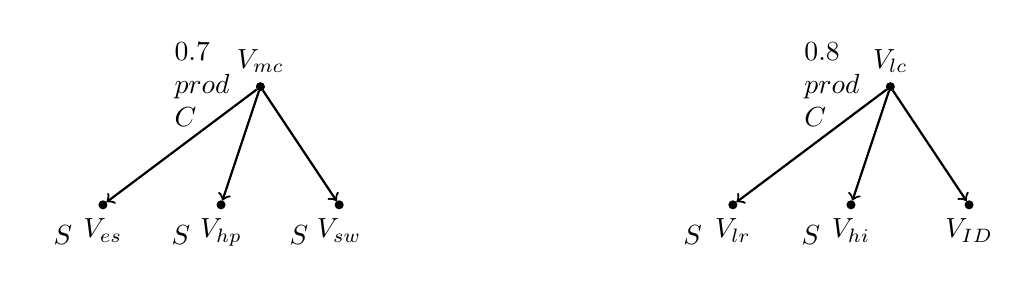
\begin{tikzpicture}[yscale=-1,
place/.style={circle,draw=black, fill=black, inner sep=0pt, 
              minimum size=1mm}]

  \node[place] (1st) at (2, 0) [label=above: $V_{mc}$,
                                  label=left: 
     \begin{tabular}{l}
        $0.7$\\
        $prod$\\
        $C$\\  
     \end{tabular}
] {};
  \node[place] (2nd) at (0, 1.5) [label=below: $V_{es}$,
                                  label=left:
     \begin{tabular}{l}
        $$\\
        $$\\
        $S$\\  
     \end{tabular}
]{};
  \node[place] (3rd) at (1.5, 1.5)  [label=below: $V_{hp}$,
                                  label=left:
     \begin{tabular}{l}
        $$\\
        $$\\
        $S$\\  
     \end{tabular}	] {}; 
  \node[place] (4th) at (3, 1.5)   [label=below: $V_{sw}$,
                                  label=left:
     \begin{tabular}{l}
        $$\\
        $$\\
        $S$\\  
     \end{tabular}
             ] {}; 
  
  %\node (dots) at (2,1.5) {$\cdots$};
	
  \draw[->, thick] (1st) -- (2nd);
  \draw[->, thick] (1st) -- (3rd);
  \draw[->, thick] (1st) -- (4th);

\begin{scope}[xshift=8cm]
  \node[place] (1st) at (2, 0) [label=above: $V_{lc}$,
                                  label=left: 
     \begin{tabular}{l}
        $0.8$\\
        $prod$\\
        $C$\\  
     \end{tabular}
] {};

  \node[place] (2nd) at (0, 1.5) [label=below: $V_{lr}$,
                                  label=left:
     \begin{tabular}{l}
        $$\\
        $$\\
        $S$\\  
     \end{tabular}
]{};
  \node[place] (3rd) at (1.5, 1.5)  [label=below: $V_{hi}$,
                                  label=left:
     \begin{tabular}{l}
        $$\\
        $$\\
        $S$\\  
     \end{tabular}	] {}; 
  \node[place] (4th) at (3, 1.5)   [label=below: $V_{ID}$,
                                  label=left:
     \begin{tabular}{l}
        $$\\
        $$\\
       % $R$\\  
     \end{tabular}
             ] {}; 

%  \node (dots) at (1,1.5) {$\cdots$};
	
\draw[->, thick] (1st) -- (2nd);
  \draw[->, thick] (1st) -- (3rd);
  \draw[->, thick] (1st) -- (4th);

\end{scope}

);
\end{tikzpicture}
\end{center}
\caption{Predicate trees after one level of expansion in \textit{SBM}}
\label{fig:res2}
\end{figure}

After the first expansion is done, again an identity predicate is introduced for the missing leaf node in the predicate tree with the root \textit{livable\_city}. The problem arise in this step. As we have discussed before, \textit{SBM} makes a filtering of the node-pairs before the next expansion, with respect to the similarity proximities of the pairs in this level. And once again as we have mentioned, this as most of the information hidden in the lower levels is not apparent to the algorithm yet, filtering can cause neglecting some important paths of the tree.

For instance at this point, between the node pairs, only a similarity relation between the predicates \textit{literacy\_rate} and \textit{social\_welfare} is defined. The algorithm continues expanding, via selecting the \textit{middle set} with the highest similarity value at the current value as the \textit{decision middle set}. So in this example, at the first level \textit{$M_{ds}$} = \{ (\textit{$V_{sw }$} , \textit{$V_{lr}$} ), (\textit{$V_{hp }$} , \textit{$V_{ID}$} ) \}  or \textit{$M_{ds}$} = \{ (\textit{$V_{sw }$} , \textit{$V_{lr}$} ), (\textit{$V_{es }$} , \textit{$V_{ID}$} ) \}  as they prove to be the best of the \textit{$M_{s}$} sets.


% --------------------------------------------------------------------------------------------




\begin{figure}[h!]
\begin{center}
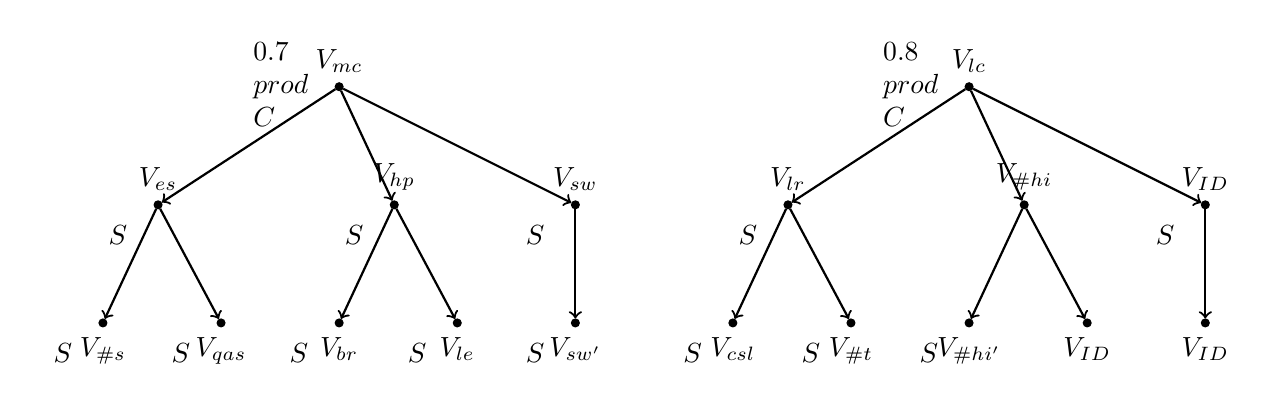
\begin{tikzpicture}[yscale=-1,
place/.style={circle,draw=black, fill=black, inner sep=0pt, 
              minimum size=1mm}]

  \node[place] (1st) at (3, 0) [label=above: $V_{mc}$,
                                  label=left: 
     \begin{tabular}{l}
        $0.7$\\
        $prod$\\
        $C$\\  
     \end{tabular}
] {};
  \node[place] (2nd) at (0.7, 1.5) [label=above: $V_{es}$,
                                  label=left:
     \begin{tabular}{l}
        $$\\
        $$\\
        $S$\\  
     \end{tabular}
]{};
  \node[place] (3rd) at (3.7, 1.5)  [label=above: $V_{hp}$,
                                  label=left:
     \begin{tabular}{l}
        $$\\
        $$\\
        $S$\\  
     \end{tabular}	] {}; 
  \node[place] (4th) at (6, 1.5)   [label=above: $V_{sw}$,
                                  label=left:
     \begin{tabular}{l}
        $$\\
        $$\\
        $S$\\  
     \end{tabular}
             ] {}; 
             
             
             
             
             
               \node[place] (5th) at (0, 3) [label=below: $V_{\#s}$,
                                  label=left:
     \begin{tabular}{l}
        $$\\
        $$\\
        $S$\\  
     \end{tabular}
]{};  

\node[place] (6th) at (1.5, 3) [label=below: $V_{qas}$,
                                  label=left:
     \begin{tabular}{l}
        $$\\
        $$\\
        $S$\\  
     \end{tabular}
]{};
  
  
                 \node[place] (7th) at (3, 3) [label=below: $V_{br}$,
                                  label=left:
     \begin{tabular}{l}
        $$\\
        $$\\
        $S$\\  
     \end{tabular}
]{};  

\node[place] (8th) at (4.5, 3) [label=below: $V_{le}$,
                                  label=left:
     \begin{tabular}{l}
        $$\\
        $$\\
        $S$\\  
     \end{tabular}
]{};
  
  
  
                 \node[place] (9th) at (6, 3) [label=below: $V_{sw'}$,
                                  label=left:
     \begin{tabular}{l}
        $$\\
        $$\\
        $S$\\  
     \end{tabular}
]{};  


  
  
  
  
  
  %\node (dots) at (2,1.5) {$\cdots$};
	
  \draw[->, thick] (1st) -- (2nd);
  \draw[->, thick] (1st) -- (3rd);
  \draw[->, thick] (1st) -- (4th);
    \draw[->, thick] (2nd) -- (5th);
      \draw[->, thick] (2nd) -- (6th);
          \draw[->, thick] (3rd) -- (7th);
      \draw[->, thick] (3rd) -- (8th);
          \draw[->, thick] (4th) -- (9th);

\begin{scope}[xshift=8cm]
    \node[place] (1st) at (3, 0) [label=above: $V_{lc}$,
                                  label=left: 
     \begin{tabular}{l}
        $0.8$\\
        $prod$\\
        $C$\\  
     \end{tabular}
] {};
  \node[place] (2nd) at (0.7, 1.5) [label=above: $V_{lr}$,
                                  label=left:
     \begin{tabular}{l}
        $$\\
        $$\\
        $S$\\  
     \end{tabular}
]{};
  \node[place] (3rd) at (3.7, 1.5)  [label=above: $V_{\#hi}$,
                                  label=left:
     \begin{tabular}{l}
        $$\\
        $$\\
       % $S$\\  
     \end{tabular}	] {}; 
  \node[place] (4th) at (6, 1.5)   [label=above: $V_{ID}$,
                                  label=left:
     \begin{tabular}{l}
        $$\\
        $$\\
        $S$\\  
     \end{tabular}
             ] {}; 
             
             
             
             
             
               \node[place] (5th) at (0, 3) [label=below: $V_{csl}$,
                                  label=left:
     \begin{tabular}{l}
        $$\\
        $$\\
        $S$\\  
     \end{tabular}
]{};  

\node[place] (6th) at (1.5, 3) [label=below: $V_{\#t}$,
                                  label=left:
     \begin{tabular}{l}
        $$\\
        $$\\
        $S$\\  
     \end{tabular}
]{};
  
  
                 \node[place] (7th) at (3, 3) [label=below: $V_{\#hi'}$,
                                  label=left:
     \begin{tabular}{l}
        $$\\
        $$\\
        $S$\\  
     \end{tabular}
]{};  

\node[place] (8th) at (4.5, 3) [label=below: $V_{ID}$,
                                  label=left:
     \begin{tabular}{l}
        $$\\
        $$\\
       % $S$\\  
     \end{tabular}
]{};
  
  
  
                 \node[place] (9th) at (6, 3) [label=below: $V_{ID}$,
                                  label=left:
     \begin{tabular}{l}
        $$\\
        $$\\
    %    $S$\\  
     \end{tabular}
]{};  


  \draw[->, thick] (1st) -- (2nd);
  \draw[->, thick] (1st) -- (3rd);
  \draw[->, thick] (1st) -- (4th);
    \draw[->, thick] (2nd) -- (5th);
      \draw[->, thick] (2nd) -- (6th);
          \draw[->, thick] (3rd) -- (7th);
      \draw[->, thick] (3rd) -- (8th);
          \draw[->, thick] (4th) -- (9th);





\end{scope}

);
\end{tikzpicture}
\end{center}
\caption{Predicate trees after two levels of expansion in \textit{SBM}}
\label{fig:res2}
\end{figure}




\

However this local optimization approach eliminates other fruitful pair combinations such as \textit{social\_welfare} and \textit{educated\_society}. In \textit{Figure 6} this pair corresponds to the left subtrees of the main predicate trees. These prove to be the most similar subconcepts of the two as there are two leaf node pairs for which the similarity relation is defined via values \textit{0.9} and \textit{0.85}. 

All in all, wrong choice for filtering causes comparing wrong pairs of subpredicates in the end and thus a distorted final similarity degree between the predicates of interest.


% --------------------------------------------------------------------------------------------

\subsection{Shared Similarity Concepts}
\label{sharedSim2}

In section \ref{sharedSim}, we had discussed the incapability of the \textit{SBM} realizing the information where a specific concept is included in more then one similarity relations as the methodology seeks for a one to one mapping between the subconcepts of the main predicates.  Our algorithm does not suffer from the same problem as it may collect and process all distinct information from each different fuzzy similarity rules.

\begin{ex}
Let us once again observe the following simple program:
\begin{center}
\begin{tabular}{l l}
$touristic\_place:$  & $(Land)$\\

$nice\_destinationt:$  & $(Land)$\\

$cultural\_venues:$  & $(Sight)$\\

$natural\_wonders:$  & $(Sight)$\\

$many\_sights:$  & $(Sight)$\\

$good\_weather:$  & $(Temperature)$\\

\end{tabular}
\end{center}
\begin{tabular}{l l l}
$touristic\_place(X)$ & $\stackrel{1.0,.}{\longleftarrow} prod$ & $cultural\_venues(X), natural\_wonders(X).$\\

$nice\_destination(X)$ & $\stackrel{1.0,.}{\longleftarrow} prod$ & $good\_weather(X), many\_sights(X).$\\


\end{tabular}
\[Sim(cultural\_venues, many\_sights) = 0.7\]
\[Sim(natural\_wonders, many\_sights) = 0.7\]
\end{ex}

In section \ref{sharedSim} we had proved that the algorithm is bound to miss one of the similarity relations and thus the corresponding evaluation algorithm could not utilize the complete data.

Let us tackle the problem with our methodology:

$cred_{p_{1}}$ = 1 , $cred_{p_{2}}$ = 1,  \emph{OP} = \textit{prod},  \textit{pm} = \{ (cultural\_venues, many\_sights), (natural\_wonders, many\_sights)\}, \textit{sm} = \{\textit{0.7, 0.7}\}, \textit{n} = 2.

And finally the evaluation:
\begin{equation}\label{eq:sdE3}
\begin{split}
\textit{$sd(p_{1}, p_{2})$} &=   (1-\lvert  \textit{$cred_{p_{1}}$} - \textit{$cred_{p_{2}}$}  \rvert) \textbf{\emph{OP}} (\frac{\sum_{i=1}^{n} sm_i}{n})\\
 &=   (1-\lvert  1 - 1  \rvert) . (\frac{0.7 + 0.7}{2}) \\
&\cong{\textbf{0.7}}
 \end{split} 
\end{equation}

As foreseen, the search algorithm were able to realize both of the similarity relations and hence the evaluation algorithm had concluded the accurate similarity degree, which is $0.7$ for the case.



%\begin{comment}

\begin{figure}[h!]
\begin{center}
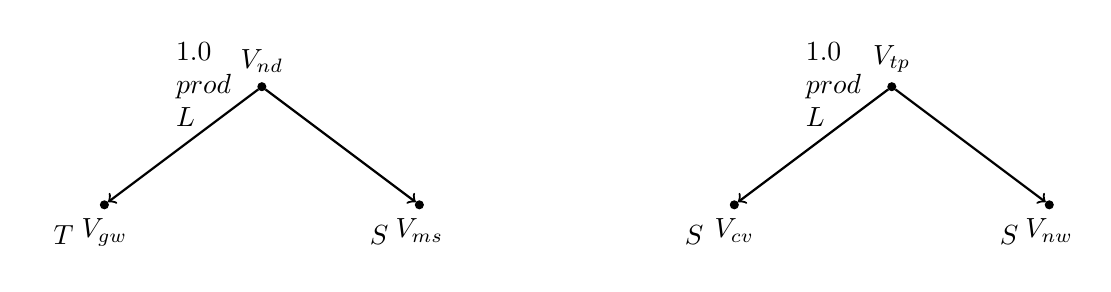
\begin{tikzpicture}[yscale=-1,
place/.style={circle,draw=black, fill=black, inner sep=0pt, 
              minimum size=1mm}]

  \node[place] (1st) at (2, 0) [label=above: $V_{nd}$,
                                  label=left: 
     \begin{tabular}{l}
        $1.0$\\
        $prod$\\
        $L$\\  
     \end{tabular}
] {};
  \node[place] (2nd) at (0, 1.5) [label=below: $V_{gw}$,
                                  label=left:
     \begin{tabular}{l}
        $$\\
        $$\\
        $T$\\  
     \end{tabular}
]{};
  \node[place] (3rd) at (4, 1.5)  [label=below: $V_{ms}$,
                                  label=left:
     \begin{tabular}{l}
        $$\\
        $$\\
        $S$\\  
     \end{tabular}	] {}; 
 

  %\node (dots) at (2,1.5) {$\cdots$};
	
  \draw[->, thick] (1st) -- (2nd);
  \draw[->, thick] (1st) -- (3rd);

\begin{scope}[xshift=8cm]
  \node[place] (1st) at (2, 0) [label=above: $V_{tp}$,
                                  label=left: 
     \begin{tabular}{l}
        $1.0$\\
        $prod$\\
        $L$\\  
     \end{tabular}
] {};

  \node[place] (2nd) at (0, 1.5) [label=below: $V_{cv}$,
                                  label=left:
     \begin{tabular}{l}
        $$\\
        $$\\
        $S$\\  
     \end{tabular}
]{};
  \node[place] (3rd) at (4, 1.5)  [label=below: $V_{nw}$,
                                  label=left:
     \begin{tabular}{l}
        $$\\
        $$\\
        $S$\\  
     \end{tabular}	] {}; 

             ] {};     

%  \node (dots) at (1,1.5) {$\cdots$};
	
\draw[->, thick] (1st) -- (2nd);
  \draw[->, thick] (1st) -- (3rd);
\end{scope}

);
\end{tikzpicture}
\end{center}
\caption{Predicate trees for \textit{nice\_destination} and \textit{touristic\_place}}
\label{fig:placeJust}
\end{figure}

%\end{comment}
% --------------------------------------------------------------------------------------------


\subsection{Credibility of Similarity Relations}
\label{credSim}

The domain of interest can be enriched by computing not only the similarity value between predicates, but also the credibility value this similarity has via the introduction of the \textit{fuzzy similarity predicates} with \textit{fuzzy credibility values}. 

In the previous research all fuzzy similarity relations are defined without credibility values as if we assume that the similarity computed was always the expected one.
So the following type of notation,

\[Sim(good\_technique,  swift\_shot) = 0.7\]

can be replaced by:
\begin{center}
\begin{tabular}{l l}
$Sim(good\_technique,  swift\_shot)$ & $\stackrel{1.0}{\longleftarrow} 0.7.$\\
\end{tabular}
\end{center}

This extension could be handled by our algorithm with just a small modification in the evaluation equation. In the part where the similarity degree of the collected pairs' are summed, we should normalize each of these values by the rule's credibility. Thus the algorithm is re-written as:

\begin{equation}\label{eq:sd2}
\textit{$sd(p_{1}, p_{2})$} =   (1-\lvert  \textit{$cred_{p_{1}}$} - \textit{$cred_{p_{2}}$}  \rvert) \textbf{\emph{OP}} (\frac{\sum_{i=1}^{n} (sm_i \times w_i)}{n})
\end{equation}


\begin{ex}
Let's revisit Ex. 2.3., but this time suppose we are sure of the similarity  relations with credibility values of 0.7 and 0.6 respectively. 
\begin{center}
\begin{tabular}{l l}
$classy\_restaurant:$  & $(Restaurant)$\\

$good\_restaurant:$  & $(Restaurant)$\\

$well\_trained\_waiters:$  & $(Restaurant)$\\

$expensive\_inventory:$  & $(Restaurant)$\\

$has\_good\_service:$  & $(Restaurant)$\\

$has\_healthy\_food:$  & $(Restaurant)$\\

$has\_tasty\_food:$  & $(Restaurant)$\\

$has\_nice\_surroundings:$  & $(Restaurant)$\\

$has\_high\_reputation:$  & $(Restaurant)$\\
\end{tabular}
\end{center}
\begin{tabular}{l l l}
$classy\_restaurant(X)$ & $\stackrel{1.0,.}{\longleftarrow} prod$ & $well\_trained\_waiters(X), expensive\_inventory(X).$\\

$good\_restaurant(X)$ & $\stackrel{0.95,.}{\longleftarrow} prod$ & $has\_healthy\_food(X), has\_good\_service(X), has\_tasty\_food(X),$\\ 
%$has\_nice\_surroundings(X), $ & $has\_nice\_surroundings(X),$ $has\_nice\_surroundings(X), $\\
$ $ & $$ & $has\_nice\_surroundings(X), has\_high\_reputation(X).$\\

\end{tabular}

\begin{tabular}{l l}
$Sim(well\_trained\_waiters, has\_good\_service)$ & $\stackrel{0.7}{\longleftarrow} 0.9.$\\
$Sim(expensive\_inventory, has\_nice\_surroundings)$ & $\stackrel{0.6}{\longleftarrow} 0.8.$\\
\end{tabular}

\end{ex}

The only change in our search procedure is that, now the collected similarity values are stored together with their associated credibility value.

Thus the new result from the modified evaluation algorithms follows as:

\begin{equation}\label{eq:sdE5}
\begin{split}
\textit{$sd(p_{1}, p_{2})$} &=   (1-\lvert  \textit{$cred_{p_{1}}$} - \textit{$cred_{p_{2}}$}  \rvert) \textbf{\emph{OP}} (\frac{\sum_{i=1}^{n} (sm_i \times w_i)}{n})\\
 &=   (1-\lvert  0.95 - 1  \rvert) . (\frac{(0.9\times 0.7) + (0.8 \times 0.6)}{2}) \\
&\cong{\textbf{0.53}}
 \end{split} 
\end{equation}

Note that the evaluated similarity value decreased to \textit{0.53} from it's original value of \textit{0.81}. This was expected as the similarity  relations' credibility decreased to \textit{0.7} and \textit{0.6} from \textit{1.0}, since they used to be treated as if they were facts. 

\end{document}